\chapter{Gesti\'{o}n del proyecto}

En este cap\'{i}tulo se presenta todo lo relacionado con la gesti\'{o}n del proyecto realizado: EDT (Estructura de descomposici\'{o}n del trabajo), la gesti\'{o}n del alcance, de los costes, de tiempo y de los riesgos.

\section{EDT}

\begin{figure}[H]
	\captionsetup{justification=centering}
	\centering
	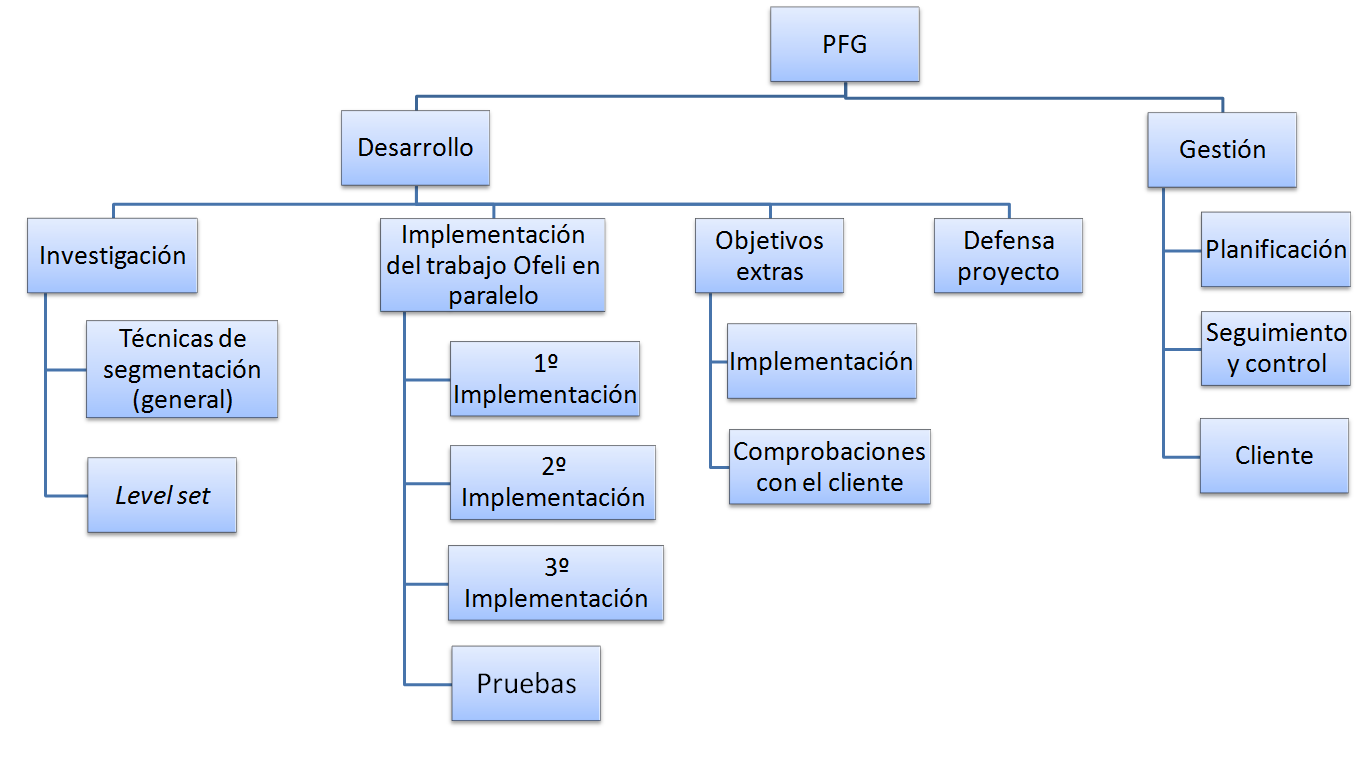
\includegraphics[width=1.2\textwidth]{./imagenes/EDT}
	\caption{EDT}	
	\label{EDT}
\end{figure}


\section{Gesti\'{o}n del alcance}\label{alcance}
 
El alcance inicial de este proyecto est\'{a} descrito en la secci\'{o}n \ref{obj-cliente}, sin embargo, \'{e}ste puede verse alterado en base al primer riesgo identificado que se explicar\'{a} en la secci\'{o}n \ref{riesgos}. Por lo tanto, se ha definido un alcance alternativo como recurso en caso de que se diera dicho riesgo.

\subsubsection{Nuevos objetivos a cumplir dado el primer riesgo}

\begin{enumerate}
	\item Se har\'{i}a un estudio de las diferentes t\'{e}cnicas de segmentaci\'{o}n existentes de una forma m\'{a}s exhaustiva, es decir, se estudiar\'{i}an las diferentes optimizaciones o mejoras que se hayan realizado para cada t\'{e}cnica de segmentaci\'{o}n. 
	\item Se buscar\'{i}an implementaciones ya realizadas de manera eficiente de cada t\'{e}cnica de segmentaci\'{o}n, de manera que se hiciera una tabla completa con las ventajas y las desventajas de cada una, poder probar estas implementaciones con diferentes im\'{a}genes si se pudiera, y comparar los resultados de la segmentaci\'{o}n, gr\'{a}ficas de los tiempos de ejecuci\'{o}n y rendimientos de cada una de \'{e}stas. 
	\item Encontrada la mejor optimizaci\'{o}n de alguna de las diferentes t\'{e}cnicas se podr\'{i}a proceder a realizar su implementaci\'{o}n eficaz, si la t\'{e}cnica no es muy compleja, en diferentes arquitecturas como MPP, SMP o en GPUs. Se comparar\'{i}a lo realizado con las diferentes opciones encontradas en la anterior idea. 
	\item En funci\'{o}n de la carga de las anteriores ideas, se podr\'{i}a proceder a realizar alguna implementaci\'{o}n de otro algoritmo de segmentaci\'{o}n m\'{a}s con el mismo fin de realizar una comparativa con otras t\'{e}cnicas y analizar rendimientos.
\end{enumerate}
 
\

\section{Gesti\'{o}n de los costes}

El coste de este proyecto ha sido \'{u}nicamente la dedicaci\'{o}n de horas dedicadas en su realizaci\'{o}n. En la tabla \ref{dedicacionTemporal} se puede observar la dedicaci\'{o}n atribuida a cada tarea.
 
\

\begin{table}[H]
	\captionsetup{justification=centering}
	\centering
	\begin{tabular}{clcp{20mm}p{20mm}M{20mm}}\toprule
		{\bf Categor\'{i}a}                						& {\bf Tarea}            							   	& {\bf Dedicaci\'{o}n (h)} \\ \midrule\midrule
		 \multirow{2}{*}{Investigaci\'{o}n} 					& T\'{e}cnicas de segmentaci\'{o}n (general)           	& 28                   \\  \cmidrule(l){2-3}
		& {\it Level set}                             			& 11                   \\ \midrule \midrule
		& Revisi\'{o}n c\'{o}digo Ofeli (ver factibilidad)     	& 2                    \\ \cmidrule(l){2-3}
		& Familiarizaci\'{o}n c\'{o}digo Ofeli                 	& 5                    \\ \cmidrule(l){2-3}
		& Dise\~{n}o de estrategia de paralelizaci\'{o}n       	& 6                    \\ \cmidrule(l){2-3}		\multirow{2}{*}{Programaci\'{o}n} & Extracci\'{o}n GUI de Ofeli                      & 8                    \\  \cmidrule(l){2-3}
		& Implementaci\'{o}n paralela                      		& 94                   \\ \cmidrule(l){2-3}
		& Preparaci\'{o}n de las m\'{a}quinas para las pruebas	& 4                    \\ \cmidrule(l){2-3}
		& Realizaci\'{o}n de pruebas                       		& 16                   \\ \cmidrule(l){2-3}
		& Implementaci\'{o}n objetivos secundarios         		& 35                   \\ \midrule \midrule
		& Recogida de requisitos                       			& 5                    \\ \cmidrule(l){2-3}
		Cliente & Reuniones de seguimiento y control (cliente)          	& 7                   \\ \cmidrule(l){2-3}
		& Reuni\'{o}n final                                		& 3                    \\ \midrule \midrule
        & Aprendizaje \LaTeX y adaptaci\'{o}n de plantilla  	& 5                    \\ \cmidrule(l){2-3}
		& Redacci\'{o}n de memoria                         		& 112                  \\ \cmidrule(l){2-3}
		\multirow{2}{*}{Otros} & Reuniones de seguimiento y control (proyecto)         & 18                   \\ \cmidrule(l){2-3}
        & Aprendizaje C++ y repaso de Github y OpenMP  			& 7                    \\ \cmidrule(l){2-3}
        & Planificaci\'{o}n 								& 16 \\ \cmidrule(l){2-3}
        & Preparaci\'{o}n de la defensa (estimado)         		& 20                   \\ \midrule \midrule
        & \bf{TOTAL}            & \textbf{402} \\ \midrule                
	\end{tabular}
	\caption{Dedicaci\'{o}n del proyecto}	
	\label{dedicacionTemporal}	
\end{table}




\section{Gesti\'{o}n del tiempo}

El proyecto dio comienzo el d\'{i}a 8 de Enero de 2015 con el primer planteamiento del proyecto y finaliz\'{o} el 16 de Septiembre del 2015 con la defensa del proyecto. Los siguientes son los hitos m\'{a}s significativos que han tenido lugar en el desarrollo del proyecto:
 
\begin{itemize}
	\item \textbf{8 de Enero}, inicio del proyecto.
	\item \textbf{16 de Febrero},  resultados de la investigaci\'{o}n aprobados por los tutores y el cliente: aproximaci\'{o}n del level set y Ofeli.
	\item \textbf{21 de Abril}, primera Implementaci\'{o}n paralela Ofeli completa.
	\item \textbf{15 de Mayo}, segunda implementaci\'{o}n paralela.
	\item \textbf{30 de Mayo}, tercera implementaci\'{o}n paralela.
	\item \textbf{28 de Junio}, una primera versi\'{o}n provisional de la memoria del proyecto.
	\item \textbf{21 de Julio}, segunda versi\'{o}n provisional de la memoria del proyecto.
	\item \textbf{14 de Agosto}, finalizaci\'{o}n de objetivos extra del cliente.
	\item \textbf{28 de Agosto}, finalizaci\'{o}n de la memoria.
\end{itemize}




\section{Gesti\'{o}n de los riesgos}\label{riesgos}

Al inicio del proyecto se han identificado una serie de riesgos que podr\'{i}an poner en peligro el desarrollo del proyecto.

\begin{enumerate}
	\item El primer y principal riesgo del proyecto, y por lo tanto, el que mayor impacto tendr\'{i}a ser\'{i}a el no poder encontrar una soluci\'{o}n implementada de un algoritmo de segmentaci\'{o}n eficaz. La eficacia del algoritmo es necesaria de manera que se consiga la mayor precisi\'{o}n posible en la extracci\'{o}n de los objetos de la imagen.
	
	La alternativa ser\'{i}a el realizar el estudio de posibilidades en s\'{i} mismo, de manera que se ofrezca al cliente la mejor soluci\'{o}n para intentar resolver el principal objetivo del proyecto. Esta alternativa cambiar\'{i}a el alcance de este proyecto como se ha descrito en la secci\'{o}n anterior de gesti\'{o}n del alcance \ref{alcance}.
	
	\item Una vez escogido un algoritmo de segmentaci\'{o}n, encontrado una implementaci\'{o}n de dicho algoritmo, o incluso, haber podido realizar una implementaci\'{o}n propia de \'{e}ste, se define el segundo riesgo. Se buscar\'{a} realizar una soluci\'{o}n eficiente para una arquitectura SMP de lo conseguido, sin embargo, puede que no se pueda satisfacer los requisitos del cliente para una arquitectura SMP.
	
	La alternativa es realizar una implementaci\'{o}n eficiente para otras arquitecturas, como MPP o en GPUs, en cuyo caso se utilizar\'{i}a el est\'{a}ndar MPI o la librer\'{i}a CUDA respectivamente.
	
	\item El tercer y \'{u}ltimo riesgo identificado es la p\'{e}rdida de la memoria escrita o de la implementaci\'{o}n paralela realizada a lo largo del proyecto. Para evitar que pueda producirse tal situaci\'{o}n se requiere el uso de un sistema de gesti\'{o}n de versiones, en este caso, \textit{Github}. Con esta herramienta se puede realizar un sistema de \textit{backup} sencillo como gesti\'{o}n de este riesgo. La memoria con todos sus documentos se guardar\'{a} diariamente en el repositorio de \textit{Github} de manera que en caso de p\'{e}rdida se pueda recuperar los avances realizados hasta el d\'{i}a anterior. La implementaci\'{o}n se crear\'{a} en forma de versiones en las que se le ir\'{a}n a\~{n}adiendo funcionalidades extras en cada versi\'{o}n. Cada una de estas versiones se subir\'{a}n a la plataforma \textit{Github} del autor de esta memoria \cite{gitHub1}. 
	
	La soluci\'{o}n a este \'{u}ltimo riesgo es pr\'{a}cticamente inmediata al tener realizados los \textit{backups} de todo lo realizado. En caso de p\'{e}rdida de la documentaci\'{o}n, se perder\'{i}a un d\'{i}a de avances, por lo que no supone mucho coste. En caso de p\'{e}rdida de la implementaci\'{o}n se tendr\'{a}n que volver a realizar los cambios desde una versi\'{o}n anterior, tarea que, si se guarda cada vez que se realiza un peque\~{n}o avance, no supondr\'{a} un sobrecoste muy grande.
	
\end{enumerate}